\documentclass{jarticle}
\usepackage[top=20truemm,bottom=15truemm,left=20truemm,right=20truemm]{geometry}
\usepackage{jlisting, listings, here}
\usepackage[dvipdfmx]{graphicx}
\makeatletter
\def\maketitle{%
\null
\thispagestyle{empty}%
\vfill
\begin{center}\leavevmode
\normalfont
{\LARGE \@title\par}%
\vskip 1cm
{\Large \@author\par}%
\vskip 1cm
{\Large \@date\par}%
\end{center}%
\vfill
\null
\@thanks%\vfil\null
\cleardoublepage
}
\makeatother
\lstset{language=c,
basicstyle=\ttfamily\scriptsize,
commentstyle=\textit,
classoffset=1,
keywordstyle=\bfseries,
frame=tRBl,
framesep=5pt,
showstringspaces=false,
stepnumber=1,
numberstyle=\tiny,
tabsize=2,
numbers = left,
stepnumber=1
}
\title{ソフトウェア演習V 課題4}
\author{15122013 尾持涼介}
\date{提出日:2018年2月9日}

\begin{document}
\maketitle

\section{作成したプログラムの設計情報}
\subsection{全体構成}
各ファイルで記述した関数は以下の通りである。
\begin{itemize}
  \item main.c
  \begin{itemize}
    \item main関数
    \item void error(char *mes)
  \end{itemize}
  \item scan.c
  \begin{itemize}
    \item int init\_scan(char *filename)
    \item int keyword\_search(char *string)
    \item int scan()
    \item int get\_linenum()
    \item void end\_scan()
  \end{itemize}
  \item prettyprinter.c
  \begin{itemize}
    \item int parse\_program()
    \item int block(int label)
    \item int var\_decl()
    \item int var\_names()
    \item int type()
    \item int ar\_type()
    \item int sub\_decl()
    \item int form\_para()
    \item int fukugou(int label)
    \item int statement(int label)
    \item int bunki(int label)
    \item int kurikaeshi(int label)
    \item int call\_st(int label)
    \item int exp\_narabi()
    \item int dainyu(int label)
    \item int var()
    \item int shiki()
    \item int simple()
    \item int kou()
    \item int inshi()
    \item int input\_st(int label)
    \item int output\_st(int label)
    \item int shitei()
    \item int get\_inlabel()
    \item void lib()
  \end{itemize}
  \item crossreferencer.c
  \begin{itemize}
    \item void init\_idtab()
    \item struct ID *search\_globalidtab(char *np)
    \item struct ID *search\_localidtab(char *np)
    \item int globalid\_def()
    \item int procedure\_def()
    \item int globalid\_ref(char *np)
    \item int localid\_def()
    \item int localid\_ref(char *np)
    \item int type\_mem(struct ID *p)
    \item void joint\_localtoglobal()
    \item void release\_idtab(struct ID *p)
  \end{itemize}
\end{itemize}
次に、各関数の呼び出し関係、データ参照関係について述べる。
\begin{itemize}
  \item main.c
  \begin{itemize}
    \item main関数内
    \begin{itemize}
      \item init\_scan()関数を呼び出し
      \item scan()関数を呼び出し
      \item parse\_program()関数を呼び出し
      \item end\_scan()関数を呼び出し
    \end{itemize}
    \item error関数内
    \begin{itemize}
      \item get\_linenum()関数を参照
    \end{itemize}
  \end{itemize}
  \item scan.c
  \begin{itemize}
    \item init\_scan()関数内
    \begin{itemize}
      \item init\_idtab()関数を呼び出し
    \end{itemize}
    \item scan()関数内
    \begin{itemize}
      \item keyword\_search()関数を呼び出し
      \item error()関数を呼び出し
    \end{itemize}
    \item end\_scan()関数内
    \begin{itemize}
      \item release\_idtab()関数を呼び出し
    \end{itemize}
  \end{itemize}
  \item prettyprinter.c
  \begin{itemize}
    \item parse\_program()関数内
    \begin{itemize}
      \item error()関数を呼び出し
      \item scan()関数を呼び出し
      \item get\_inlabel()関数を呼び出し
      \item block()関数を呼び出し
      \item lib()関数を呼び出し
    \end{itemize}
    \item block()関数内
    \begin{itemize}
      \item var\_decl()関数を呼び出し
      \item sub\_decl()関数を呼び出し
      \item fukugou()関数を呼び出し
    \end{itemize}
    \item var\_decl()関数内
    \begin{itemize}
      \item scan()関数を呼び出し
      \item var\_names()関数を呼び出し
      \item  error()関数を呼び出し
      \item type()関数を呼び出し
      \item globalid\_def()関数を呼び出し
      \item localid\_def()関数を呼び出し
    \end{itemize}
    \item var\_names()関数内
    \begin{itemize}
      \item error()関数を呼び出し
      \item scan()関数を呼び出し
    \end{itemize}
    \item type()関数内
    \begin{itemize}
      \item scan()関数を呼び出し
      \item ar\_type()関数を呼び出し
      \item error()関数を呼び出し
    \end{itemize}
    \item ar\_types()関数内
    \begin{itemize}
      \item scan()関数を呼び出し
      \item error()関数を呼び出し
    \end{itemize}
    \item sub\_decl()関数内
    \begin{itemize}
      \item scan()関数を呼び出し
      \item error()関数を呼び出し
      \item procedure\_def()関数を呼び出し
      \item form\_para()関数を呼び出し
      \item var\_decl()関数を呼び出し
      \item fukugou()関数を呼び出し
      \item joint\_localtoglobal()関数の呼び出し
    \end{itemize}
    \item form\_para()関数内
    \begin{itemize}
      \item scan()関数を呼び出し
      \item var\_names()関数を呼び出し
      \item error()関数を呼び出し
      \item type()関数を呼び出し
      \item localid\_def()関数を呼び出し
    \end{itemize}
    \item fukugou()関数内
    \begin{itemize}
      \item error()関数を呼び出し
      \item scan()関数を呼び出し
      \item statement()関数を呼び出し
    \end{itemize}
    \item statemen()関数内
    \begin{itemize}
      \item dainyu()関数を呼び出し
      \item bunki()関数を呼び出し
      \item kurikaeshi()関数を呼び出し
      \item scan()関数を呼び出し
      \item call\_st()関数を呼び出し
      \item input\_st()関数を呼び出し
      \item output\_st()関数を呼び出し
      \item fukugou()関数を呼び出し
    \end{itemize}
    \item bunki()関数内
    \begin{itemize}
      \item scan()関数を呼び出し
      \item shiki()関数を呼び出し
      \item error()関数を呼び出し
      \item get\_inbabel()関数を呼び出し
      \item statement()関数を呼び出し
    \end{itemize}
    \item kurikaeshi()関数内
    \begin{itemize}
      \item scan()関数を呼び出し
      \item shiki()関数を呼び出し
      \item error()関数を呼び出し
      \item get\_inlabel()関数を呼び出
      \item statement()関数を呼び出し
    \end{itemize}
    \item call\_st()関数内
    \begin{itemize}
      \item scan()関数を呼び出し
      \item error()関数を呼び出し
      \item globalid\_ref()関数を呼び出し
      \item localid\_ref()関数を呼び出し
      \item exp\_narabi()関数を呼び出し
    \end{itemize}
    \item exp\_narabi()関数内
    \begin{itemize}
      \item shiki()関数を呼び出し
      \item error()関数を呼び出し
      \item get\_inlabel()関数を呼び出し
    \end{itemize}
    \item dainyu()関数内
    \begin{itemize}
      \item var()関数を呼び出し
      \item error()関数を呼び出し
      \item scan()関数を呼び出し
      \item shiki()関数を呼び出し
    \end{itemize}
    \item var()関数内
    \begin{itemize}
      \item error()関数を呼び出し
      \item globalid\_ref()関数を呼び出し
      \item localid\_ref()関数を呼び出し
      \item scan()関数を呼び出し
      \item shiki()関数を呼び出し
    \end{itemize}
    \item shiki()関数内
    \begin{itemize}
      \item simple()関数を呼び出し
      \item scan()関数を呼び出し
      \item get\_inlabel()関数を呼び出し
    \end{itemize}
    \item simple()関数内
    \begin{itemize}
      \item kou()関数を呼び出し
      \item error()関数を呼び出し
      \item scan()関数を呼び出し
      \item error()関数を呼び出し
    \end{itemize}
    \item kou()関数内
    \begin{itemize}
      \item inshi()関数を呼び出し
      \item error()関数を呼び出し
      \item scan()関数を呼び出し
    \end{itemize}
    \item inshi()関数内
    \begin{itemize}
      \item var()関数を呼び出し
      \item scan()関数を呼び出し
      \item shiki()関数を呼び出し
      \item error()関数を呼び出し
      \item inshi()関数を呼び出し
    \end{itemize}
    \item input\_st()関数内
    \begin{itemize}
      \item scan()関数を呼び出し
      \item var()関数を呼び出し
      \item error()関数を呼び出し
    \end{itemize}
    \item output\_st()関数内
    \begin{itemize}
      \item scan()関数を呼び出し
      \item shitei()関数を呼び出し
      \item error()関数を呼び出し
    \end{itemize}
    \item shitei()関数内
    \begin{itemize}
      \item scan()関数を呼び出し
      \item get\_inlabel()関数を呼び出し
      \item shiki()関数を呼び出し
      \item error()関数を呼び出し
    \end{itemize}
  \end{itemize}
  \item crossreferencer.c内
  \begin{itemize}
    \item globalid\_def()関数内
    \begin{itemize}
      \item error()関数を呼び出し
      \item get\_linenum()関数を呼び出し
      \item type\_mem()関数を呼び出し
    \end{itemize}
    \item procedure\_def()関数内
    \begin{itemize}
      \item error()関数を呼び出し
      \item get\_linenum()関数を呼び出し
      \item type\_mem()関数を呼び出し
    \end{itemize}
    \item globalid\_ref()関数内
    \begin{itemize}
      \item search\_globalidtab()関数を呼び出し
      \item get\_linenum()関数を呼び出し
      \item error()関数を呼び出し
    \end{itemize}
    \item lobalid\_def()関数内
    \begin{itemize}
      \item error()関数を呼び出し
      \item type\_mem()関数を呼び出し
      \item get\_linenum()関数を呼び出し
    \end{itemize}
    \item localid\_ref()関数内
    \begin{itemize}
      \item search\_localidtab()関数を呼び出し
      \item error()関数を呼び出し
      \item get\_linenum()関数を呼び出し
      \item search\_globalidtab()関数を呼び出し
    \end{itemize}
    \item type\_mem()関数内
    \begin{itemize}
      \item error()関数を呼び出し
    \end{itemize}
    \item joint\_localtoglobal関数内
    \begin{itemize}
      \item error()関数を呼び出し
    \end{itemize}
    \item release\_idtab()関数内
    \begin{itemize}
      \item release\_idtab()関数を呼び出し(再帰呼出し)
      \item init\_idtab()関数を呼び出し
    \end{itemize}
  \end{itemize}
\end{itemize}
\subsection{各モジュールごとの構成}
出力文等で文字列が出てきたときに、その文字列を格納するための構造体を以下の図\ref{code:string}のように定義した。
\begin{figure}[H]
\begin{center}
\begin{lstlisting}
struct STRING{
char *string;
int label;
struct STRING *next;
};
\end{lstlisting}
\caption{文字列を格納するための構造体}
\label{code:string}
\end{center}
\end{figure}
なお、ここでstringは格納する文字列、labelはその文字列を定義するためのラベルの番号、nextは次の要素へのポインタである。
そしてプログラムの末尾を表す「end.」が出てきた後にまとめて出力している。

また、コード生成は適切な場所でfprintfを使って生成している。

次に使用した大域変数とその意味について述べる。

\begin{itemize}
  \item main.c内
  \begin{itemize}
    \item 課題3のレポートで説明済み
  \end{itemize}
  \item scan.c内
  \begin{itemize}
    \item int cbuf:課題2のレポートで説明済み
    \item int line\_cnt:課題2のレポートで説明済み
    \item int newline:課題2のレポートで説明済み
    \item char string\_attr[MAXSTRSIZE]:課題2のレポートで説明済み
    \item int num\_attr:課題2のレポートで説明済み
    \item FILE *fp:課題2のレポートで説明済み
    \item FILE *fpw:出力するファイルへのポインタ
  \end{itemize}
  \item prettyprinter.c内
  \begin{itemize}
    \item int arraynum:配列型の要素数を格納する変数
    \item int typenum:宣言された変数の型を表す整数を格納する。
    \item int paraflag:今調べている変数が仮引数かどうかを記憶する変数(1なら仮引数、0ならその他)。
    \item int gorl:調べている変数が大域変数か局所変数かを記憶する変数(1なら局所変数、0なら大域変数)。
    \item int arraytype:配列の要素の型を表す整数を格納する。
    \item int shikitype:「式」の型を表す整数を格納する。
    \item int shikiarraysize:「式」が配列型であるときに要素数を記憶する変数。
    \item int shikiarraytype:「式」が配列型であるときにその要素の型を記憶する変数。
    \item int vartype:「変数」の型を表す整数を格納する。
    \item int vararraysize:「変数」が配列型であるときに要素数を記憶する変数。
    \item int vararraytype:「変数」が配列型であるときにその要素の型を記憶する変数。
    \item int koutype:「項」の型を表す整数を格納する。
    \item int kouarraysize:「項」が配列型であるときに要素数を記憶する変数。
    \item int kouarraytype:「項」が配列型であるときにその要素の型を記憶する変数。
    \item int inshitype:「因子」の型を表す整数を格納する。
    \item int inshiarraysize:「因子」が配列型であるときに要素数を記憶する変数。
    \item int inshiarraytype:「因子」が配列型であるときにその要素の型を記憶する変数。
    \item int arrayflag:その前に出てきた変数が配列型かどうかを表す変数(1なら配列型、0なら標準型)
    \item int paranum:仮引数の個数を記憶する変数。
    \item int expnum:式の並びにおいて式の個数を記憶する変数。
    \item int inlab\_num:ラベル番号を格納する変数。
    \item int adflag:変数からアドレスを取り出すべきか値を取り出すべきかを表す変数(1ならアドレスを、0なら値を取り出す)。
    \item int callflag:手続き呼出し文の引数での処理であることを示す変数。
    \item int eorv:手続き呼出し文の引数が変数単体であるのか、複数の項からなる式であるのかを表す変数(1なら式、0なら変数)
    \item struct NAME *names:変数宣言部、仮引数部における変数名の並びを記憶する線形リストの先頭要素を指すポインタ。
    \item struct TYPE *paratype:仮引数の型を記憶する線形リストの先頭要素を指すポインタ。
    \item struct ID *searchp:局所変数・大域変数のリストのうち、探索した変数名の要素を指すポインタ。
    \item char token\_str[NUMOFTOKEN+1]:トークン名(キーワード名)が格納された配列。
    \item struct STRING *stringhead:文字列を格納する線形リストの先頭要素を指すポインタ。
    \item struct STRING *stringtail:文字列を格納する線形リストの末尾要素を指すポインタ。
    \item struct NAME *para:仮引数を格納する線形リストの先頭要素を指すポインタ
  \end{itemize}
  \item crossreferencer.c内
  \begin{itemize}
    \item struct ID *globalidroot:大域変数を格納する二分探索木の先頭要素を指すポインタ。
    \item struct ID *localidroot:局所変数を格納する二分探索木の先頭要素を指すポインタ。
    \item char *typename[NUMOFTYPE+1]:型名を格納した配列。
  \end{itemize}
\end{itemize}

次に各関数内で定義した変数とその意味について述べる

\begin{itemize}
  \item scan.c
  \begin{itemize}
    \item init\_scan()関数内
    \begin{itemize}
      \item char *newfile:元のファイル名の拡張子を.cslに変えたものを格納するポインタ。
      \item int lebgth:元のファイル名の長さを表す変数。
      \item int i:ループ変数
    \end{itemize}
    \item ikeyword\_search()関数内:課題1で記載済み
    \item scan()関数内
    \begin{itemize}
      \item int i:課題1で記載済み
    \end{itemize}
  \end{itemize}
  \item prettyprinter.c
  \begin{itemize}
    \item parse\_program()内
    \begin{itemize}
      \item int label;プログラムが最初に実行する部分を表すラベルを表す変数。
      \item struct STRING *p,*q:文字列を格納している線形リストを辿るためのポインタ。
    \end{itemize}
    \item var\_decl()内
    \begin{itemize}
      \item struct NAME *p:変数名が格納された線形リストを惰どるためのポインタ。
    \end{itemize}
    \item var\_names()内
    \begin{itemize}
      \item struct NAME *p:namesに追加する要素を指すポインタ。
      \item struct NAME *q:作成した要素をnamesに挿入するためにnamesをたどるポインタ。
      \item char *cp:線形リストに格納する変数名を格納するポインタ。
    \end{itemize}
    \item type()内
    \begin{itemize}
      \item int a:ar\_type()関数からの返り値を記憶する変数。
    \end{itemize}
    \item sub\_decl()関数内
    \begin{itemize}
      \item struct NAME *p, *q:仮引数を格納したリストを辿るためのポインタ
      \item int flag:その副プログラムに引数があるかどうかを表す変数。
    \end{itemize}
    \item form\_para()関数内
    \begin{itemize}
      \item struct NAME *n,*m:for文でnamesを辿るためのポインタ。
      \item struct NAME *l:仮引数を格納するリストに新たに加える要素を指すポインタ。
      \item struct TYPE *p:新たな仮引数の型情報を格納するポインタ。
      \item struct TYPE *q:pがさす要素をparatpにつなげるためのポインタ。
      \item char *cp:仮引数を格納するリストに新たに加える変数名を格納するポインタ。
    \end{itemize}
    \item bunki()関数内
    \begin{itemize}
      \item int flag:課題2で記載済み。
      \item int label1,label2:ラベル番号を表す変数。
    \end{itemize}
    \item kurikaeshi()関数内
    \begin{itemize}
      \item
      int
      flag:課題2で記載済み
      \item int label1,label2:ラベル番号を表す変数。
    \end{itemize}
    \item call\_st()関数内
    \begin{itemize}
      \item struct TYPE *q:呼び出し文で呼び出された副プログラムの仮引数の型情報を記憶する構造体の先頭要素を指すポインタ。
      \item char *callname:呼び出す副プログラムの名前を表すポインタ。
    \end{itemize}
    \item exp\_narabi()関数内
    \begin{itemize}
      \item struct TYPE *p:式の型情報を記憶する構造体の先頭要素を指すポインタ。
      \item int label;ラベル番号を表す変数。
      \item struct STRING *p;文字列を格納するリストに新たに加える要素を指すポインタ。
      \item char *cp:文字列を格納するリストに新たに加える文字列(ここでは、領域を確保するために0を格納)を格納するポインタ。
    \end{itemize}
    \item dainyu()関数内
    \begin{itemize}
      \item int type1:左辺値の型を記憶する変数。
      \item int type2:代入する式の型を記憶する変数。
    \end{itemize}
    \item var()関数内
    \begin{itemize}
      \item int arraytype:変数名が配列型の場合その要素の型を記憶する変数。
      \item int arraysize:変数名が配列型の場合その要素数を記憶する変数。
    \end{itemize}
    \item shiki()関数内
    \begin{itemize}
      \item int type1, type2:それぞれの直前で出現した単純式の型を記憶する変数。
      \item int
      arraysize1、arraysize2:それぞれの直前に出現した単純式が配列型だった場合にその要素数を記憶する変数。
      \item int
      arraytype1、arraytype2:それぞれの直前に出現した単純式が配列型だった場合にその要素の型を記憶する変数。
      \item int opr:関係演算子を記憶する変数。
      \item int label1,label2:ラベル番号を記憶する変数。
    \end{itemize}
    \item simple()関数内
    \begin{itemize}
      \item int flag:最初の項の前に+か-があるかどうかを示す変数(0ならない、1ならある)。
      \item int minusflag:最初の項の前に-があるかどうかを示す変数(0ならない、1ならある)
      \item int type1, type2:それぞれの直前に出現した項の型を記憶する変数。
      \item int kahou:加法演算子を記憶する変数。
    \end{itemize}
    \begin{itemize}
      \item int type1, type2:それぞれの直前に出現した因子の型を記憶する変数。
      \item int jouhou:情報演算子を記憶する変数。
    \end{itemize}
    \item inshi()関数内
    \begin{itemize}
      \item int type1:因子の最初に標準型がある場合にその型を記憶する変数。
    \end{itemize}
    \item input\_st()関数内
    \begin{itemize}
      \item int op:入力文を表す命令が「read」であるか「readln」であるかを記憶する変数。
    \end{itemize}
    \item output\_st()関数内
    \begin{itemize}
      \item int op:出力文を表す命令が「write」であるか「writeln」であるかを記憶する変数。
    \end{itemize}
    \item shitei()関数内
    \begin{itemize}
      \item struct STRING *p:文字列を格納するリストに新たに加える要素を指すポインタ。
      \item char *cp:文字列を格納するリストに新たに加える文字列を指すポインタ。
      \item int label:ラベル番号を表す変数。
    \end{itemize}
  \end{itemize}
  \item crossreferencer.c内
  \begin{itemize}
    \item search\_globalidtab()関数内
    \begin{itemize}
      \item struct ID *p:for文による探索のためにglobalrootを辿るポインタ。
    \end{itemize}
    \item search\_localidtab()関数内
    \begin{itemize}
      \item struct ID *p:for文による探索のためにlocalrootを辿るポインタ。
    \end{itemize}
    \item globalid\_def()関数内
    \begin{itemize}
      \item struct ID *new;新しくglobalrootにつなげる要素を指すポインタ。
      \item struct ID *p;globalidrootを辿るポインタ。
      \item struct NAME *np:namesのうちglobalidrootに登録する要素を指すポインタ。
      \item struct NAME *nq:for文でnamesを辿るためのポインタ。
    \end{itemize}
    \item procedure\_def()関数内
    \begin{itemize}
      \item struct ID *new;新しくglobalrootにつなげる要素を指すポインタ。
      \item struct ID *p;globalidrootを辿るポインタ。
      \item char *cp:新しく加える手続き名を指すポインタ。
    \end{itemize}
    \item globalid\_ref()関数内
    \begin{itemize}
      \item struct ID *p:探索した要素を指すポインタ。
      \item struct LINE *next:新たに出現した行を格納すべき要素を指すポインタ。
      \item struct LINE *prev:新たに出現した行を格納すべき要素の1つ前を指すポインタ。
      \item struct LINE *m:新たに付け加える行番号を格納した要素を指すポインタ。
    \end{itemize}
    \item localid\_def()関数内
    \begin{itemize}
      \item struct ID *new;新しくlocalrootにつなげる要素を指すポインタ。
      \item struct ID *p;locaidrootを辿るポインタ。
      \item struct NAME *np:namesのうちglobalidrootに登録する要素を指すポインタ。
      \item struct NAME *nq:for文でnamesを辿るためのポインタ。
      \item char *cp:その局所変数が定義されている手続き名を格納するポインタ。
    \end{itemize}
    \item localid\_ref()関数内
    \begin{itemize}
      \item struct ID *p:探索した要素を指すポインタ。
      \item struct LINE *next:新たに出現した行を格納すべき要素を指すポインタ。
      \item struct LINE *prev:新たに出現した行を格納すべき要素の1つ前を指すポインタ。
      \item struct LINE *m:新たに付け加える行番号を格納した要素を指すポインタ。
    \end{itemize}
    \item type\_mem()関数内
    \begin{itemize}
      \item struct TYPE *q:新しく追加する型情報を格納した要素を指すポインタ。
      \item struct TYPE *r:新しく追加する型が配列型の時の要素の型情報を格納するポインタ。
      \item struct TYPE *pt:仮引数の型情報を記憶するときにparatypeを辿るポインタ。
    \end{itemize}
    \item joint\_localtoglobal()関数内
    \begin{itemize}
      \item struct ID *x:globalrootにつなげた要素を指すポインタ
      \item struct ID **p:globalidrootを辿るためのポインタ。
      \item struct ID **q:localidrootを辿るためのポインタ
    \end{itemize}
  \end{itemize}
\end{itemize}
\subsection{各関数の外部(入出力)仕様}
ここでは、各関数の機能、引数と返り値等について説明する。
\subsubsection{main.c内で記述されている関数}
\begin{itemize}
  \item main関数:課題3で記載済み。
\item void error(char *mes):課題2で記載済み
\end{itemize}
\subsubsection{scan.c内で記述されている関数}
\begin{itemize}
  \item int init\_scan(char *filename)
  \begin{description}
  \item[機能]初期化関数。指定されたファイルを読込形式でopenし、指定されたファイルの拡張子を変更して書き込み形式でopenする。読み込むファイルの最初のトークンを読み込んでおく。
  \item[引数]char *filename:読み込みファイル名
  \item[参照・変更する大域変数]line\_cnt,newline,fp,fpw,cbuf
  \end{description}
  \item int keyword\_search(char *string):課題1で記載済み
  \item int scan():課題2で記載済み
  \item int get\_linenum():課題1で記載済み
  \item void end\_scan():課題3で記載済み
\end{itemize}
\subsubsection{prettyprinter.c内で記述した関数}
なお、以下でNORMALとERRORはそれぞれprettyprinter.c内で0、1と定義されている。
\begin{itemize}
  \item int parse\_program()
  \begin{description}
\item[機能]プログラムを解析する関数
\item[引数]なし
\item[返り値]エラーがあればERRORを、なければNORMALを返す。
\item[参照・変更する大域変数]token,fpw, stringhead
\end{description}
\item int block(int label)
\begin{description}
\item[機能]ブロックを解析する関数
\item[引数]int label:プログラムが最初に実行する場所を表すラベル番号
\item[返り値]エラーがあればERRORを、なければNORMALを返す。
\item[参照する大域変数]token,fpw
\end{description}
\item int var\_decl
\begin{description}
\item[機能]変数宣言部を解析する関数
\item[引数]なし
\item[返り値]エラーがあればERRORを、なければNORMALを返す。
\item[変更する大域変数]token
\item[参照する大域変数]gorl、token,fpw,names,typenum,procname
\end{description}
\item int var\_names()
\begin{description}
\item[機能]変数名の並びを解析する関数
\item[引数]なし
\item[返り値]エラーがあればERRORを、なければNORMALを返す。
\item[変更する大域変数]token, names
\item[参照する大域変数]string\_attr、token
\end{description}
\item int type()
\begin{description}
\item[機能]型を解析する関数
\item[引数]なし
\item[返り値]エラーがあればERRORを、なければNORMALを返す。
\item[参照・変更する大域変数]token,typenum
\end{description}
\item int ar\_type()
\begin{description}
\item[機能]配列型を解析する関数
\item[引数]なし
\item[返り値]エラーがあればERRORを、なければNORMALを返す。
\item[変更する大域変数]token、typenum、arraynum,arraytype
\item[参照する大域変数]token、string\_attr、num\_attr
\end{description}
\item int sub\_decl()
\begin{description}
\item[機能]副プログラム宣言を解析する関数
\item[引数]なし
\item[返り値]エラーがあればERRORを、なければNORMALを返す。
\item[変更する大域変数]token、gorl、localidroot、procname、para
\item[参照する大域変数]token、string\_attr、fpw、para
\end{description}
\item int form\_para()
\begin{description}
\item[機能]仮引数部を解析する関数
\item[引数]なし
\item[返り値]エラーがあればERRORを、なければNORMALを返す。
\item[変更する大域変数]token、paratype、paraflag、para
\item[参照する大域変数]names、token、typenum
\end{description}
\item int fukugou(int label)
\begin{description}
\item[機能]複合文を解析する関数
\item[引数]int label:繰り返し文の終わりを表すラベル番号
\item[返り値]エラーがあればERRORを、なければNORMALを返す。
\item[参照・変更する大域変数]token
\end{description}
\item int statement(int label)
\begin{description}
\item[機能]文を解析する関数
\item[引数]int label:繰り返し文の終わりを表すラベル番号
\item[返り値]エラーがあればERRORを、なければNORMALを返す。
\item[参照・変更する大域変数]token、fpw
\end{description}
\item int bunki(int label)
\begin{description}
\item[機能]分岐文を解析する関数
\item[引数]int label:繰り返し文の終わりを表すラベル番号なし
\item[返り値]エラーがあればERRORを、なければNORMALを返す。
\item[参照・変更する大域変数]token、indentnum
\item[参照する大域変数]fpw
\end{description}
\item int kurikaeshi(int label)
\begin{description}
\item[機能]繰り返し文を解析する関数
\item[引数]int label:繰り返し文の終わりを表すラベル番号
\item[返り値]エラーがあればERRORを、なければNORMALを返す。
\item[変更する大域変数]token、
\item[参照する大域変数]shikitype、token、fpw
\end{description}
\item int call\_st(int label)
\begin{description}
\item[機能]手続き呼び出し文を解析する関数
\item[引数]int label:繰り返し文の終わりを表すラベル番号
\item[返り値]エラーがあればERRORを、なければNORMALを返す。
\item[変更する大域変数]token、paranum、expnum、adflag、callflag
\item[参照する大域変数]gorl、token、string\_attr、procname、searchp、paranum、expnum
\end{description}
\item int exp\_narabi()
\begin{description}
\item[機能]式の並びを解析する関数
\item[引数]なし
\item[返り値]エラーがあればERRORを、なければNORMALを返す。
\item[変更する大域変数]token、expnum、eorv、stringhead、stringtail
\item[参照する大域変数]token、searchp、shikitype、eorv、fpw、stringhead
\end{description}
\item int dainyu(int label)
\begin{description}
\item[機能]代入文を解析する関数
\item[引数]int label:繰り返し文の終わりを表すラベル番号
\item[返り値]エラーがあればERRORを、なければNORMALを返す。
\item[変更する大域変数]token、adflag
\item[参照する大域変数]vartype、shikitype、token、fpw
\end{description}
\item int var()
\begin{description}
\item[機能]変数を解析する関数
\item[引数]なし
\item[返り値]エラーがあればERRORを、なければNORMALを返す。
\item[変更する大域変数]token、vartype
\item[参照する大域変数]gorl、token、string\_attr、searchp、vartype、shikitype、fpw、adflag、inputglag
\end{description}
\item int shiki()
\begin{description}
\item[機能]式を解析する関数
\item[引数]なし
\item[返り値]エラーがあればERRORを、なければNORMALを返す。
\item[変更する大域変数]token、shikitype
\item[参照する大域変数]simpletype、token、simplearraysize、simplezrraytype、fpw、arrayflag、eorv
\end{description}
\item int simple()
\begin{description}
\item[機能]単純式を解析する関数
\item[引数]なし
\item[返り値]エラーがあればERRORを、なければNORMALを返す。
\item[変更する大域変数]token、simpletype、simplearraytype、simplearraysize、eorv
\item[参照する大域変数]token、koutype、kouarraytype、kouarraysize、fpw、arrayflag
\end{description}
\item int kou()
\begin{description}
\item[機能]項を解析する関数
\item[引数]なし
\item[返り値]エラーがあればERRORを、なければNORMALを返す。
\item[変更する大域変数]token、koutype、kouarraysize、kouarraytype、eorv
\item[参照する大域変数]inshitype、token	、fpw、callflag、arrayflag
\end{description}
\item int inshi()
\begin{description}
\item[機能]因子を解析する関数
\item[引数]なし
\item[返り値]エラーがあればERRORを、なければNORMALを返す。
\item[変更する大域変数]token、inshitype、inshiarraysize、inshiarraytype、arrayflag
\item[参照する大域変数]token、、fpw、vartype、vararraysize、vararraytype、shikitype、shikiarraysize、shikiarraytype、inshitype
\end{description}
\item int input\_st(int label)
\begin{description}
\item[機能]入力文を解析する関数
\item[引数]int label:繰り返し文の終わりを表すラベル番号
\item[返り値]エラーがあればERRORを、なければNORMALを返す。
\item[変更する大域変数]token、adflag、inputflag
\item[参照する大域変数]token、vartype、fpw
\end{description}
\item int output\_st(int label)
\begin{description}
\item[機能]出力文を解析する関数
\item[引数]int label:繰り返し文の終わりを表すラベル番号
\item[返り値]エラーがあればERRORを、なければNORMALを返す。
\item[参照・変更する大域変数]token、fpw
\end{description}
\item int shitei()
\begin{description}
\item[機能]出力指定を解析する関数
\item[引数]なし
\item[返り値]エラーがあればERRORを、なければNORMALを返す。
\item[変更する大域変数]token、stringhead、stringtail
\item[参照する大域変数]shikitype、token、fpw
\end{description}
\item get\_inlabal()
\begin{description}
\item[機能]ラベルを確保する関数
\item[引数]なし
\item[返り値]確保したラベル番号
\item[参照する大域変数]inlab\_num
\end{description}
\item voidlib()
\begin{description}
\item[機能]ライブラリ部のコード生成を行う関数
\item[引数・返り値]なし
\item[参照する大域変数]fpw
\end{description}
\end{itemize}
\subsubsection{crossreferecer.c内で記述した関数}
\begin{itemize}
  \item void init\_idtab()
  \begin{description}
\item[機能]大域変数、局所変数を格納するそれぞれの二分探索木を初期化する。
\item[引数・返り値]なし
\item[参照・変更する大域変数]globalidroot、localidroot
\end{description}
\item struct ID *search\_globalidtab(char *np)
\begin{description}
\item[機能]指定された変数名・手続き名が大域変数を格納する二分探査木の中に存在するか探索する。
\item[引数]char *np:探索する変数名・手続き名
\item[返り値]指定された変数名・手続き名が二分探索木の中に存在すればその要素を指すポインタが、存在しなければNULLを返す。
\item[参照する大域変数]globalidroot
\item[変更する大域変数]なし
\end{description}
\item struct ID *search\_localidtab(char *np)
\begin{description}
\item[機能]指定された変数名が局所変数を格納する二分探索木の中に存在するか探索する。
\item[引数]char *np:探索する変数名
\item[返り値]指定された変数名が二分探索木の中に存在すればその要素を指すポインタが、存在しなければNULLを返す。
\item[参照する大域変数]localidroot
\item[変更する大域変数]なし
\end{description}
\item int globalid\_def()
\begin{description}
\item[機能]新たに宣言された大域変数とその型情報、宣言された行番号をglobalidrootに格納する。
\item[引数]なし
\item[返り値]エラーがあればERRORを、無ければNORMALを返す。
\item[参照・変更する大域変数]globalidroot、names
\end{description}
\item int procedure\_def()
\begin{description}
\item[機能]新たに宣言された手続き名とその仮引数の型情報、宣言された行番号をglobalidrootに格納する。
\item[引数]なし
\item[返り値]エラーがあればERRORを、無ければNORMALを返す。
\item[参照する大域変数]procname、globalidroot
\item[変更する大域変数]globalidroot
\end{description}
\item int globalid\_ref(char *np)
\begin{description}
\item[機能]宣言済みの大域変数が使用された場合に、その行番号をglobalidrootの該当する要素に追加する。
\item[引数]char *np:使用された変数名・手続き名
\item[返り値]エラーがあればERRORを、無ければNORMALを返す。
\item[参照・変更する大域変数]searchp、globalidroot
\end{description}
\item int localid\_def()
\begin{description}
\item[機能]新たに宣言された局所変数とその型情報、その変数が宣言された副プログラムの手続き名、宣言された行番号をglobalidrootに格納する。
\item[引数]なし
\item[返り値]エラーがあればERRORを、無ければNORMALを返す。
\item[変更する大域変数]localidroot、names
\item[参照する大域変数]localidroot、names、procname、paraflag
\end{description}
\item int localid\_ref(char *np)
\begin{description}
\item[機能]宣言済みの大域変数が使用された場合に、その行番号をglobalidrootの該当する要素に追加する。
\item[引数]char *np:使用された変数名・手続き名
\item[返り値]エラーがあればERRORを、無ければNORMALを返す。
\item[参照・変更する大域変数]searchp、localidroot
\end{description}
\item int type\_mem(struct ID *p)
\begin{description}
\item[機能]型情報をリストに格納する。
\item[引数]struct ID *p:リストの型情報を格納すべき要素を指すポインタ。
\item[返り値]エラーがあればERRORを、無ければNORMALを返す。
\item[参照する大域変数]typenum、arraytype、arraynum、paratype
\item[変更する大域変数]paratype
\end{description}
\item void joint\_localtoglobal()
\begin{description}
\item[機能]局所変数用の二分探索木を大域変数用の二分探索木につなげる。
\item[引数・返り値]なし
\item[参照する大域変数]globalidroot、localidroot
\item[変更する大域変数]globalidroot
\end{description}
\item void release\_idtab()
\begin{description}
\item[機能]大域変数用二分探索木の領域を解放する。
\item[引数・返り値]なし
\item[参照・変更する大域変数]globalidroot
\end{description}
\end{itemize}
\section{テスト情報}
\subsection{テストデータ・テスト結果}
私はまず、ブラックボックステストとして配布されたテストデータである、sample11.mpl、sample11p.mpl、sample11pp.mpl、sample12.mpl、
sample13.mpl、sample14.mpl、sampl15.mpl、sample15a.mpl、sample16.mpl、sample17.mpl、sample18.mpl、sample19p.mpl、
sample21.mpl、sample2a.mpl、sample22.mpl、
sample23.mpl、sample24.mpl、sampl25.mpl、sample25t.mpl、sample26.mpl、sample27.mpl、sample28p.mpl、sample29p.mpl、sample31p.mpl、sample33p.mpl、sample34.mpl、sample35.mplについてテストを行った。

配布されたテストデータによるテスト結果(CSLファイルとシミュレータによる実行結果)ついてはメールにより提出する。
なお、CSLファイルについては「(テストプログラム名).csl」、シミュレータによる実行結果については「(テストプログラム名).png」としている(テストプログラム名の.mplは省略)。それらをまとめて「kadai4-test.zip」
というファイルにまとめて圧縮して提出する。なお、sample21から23については、何も出力しないファイルであるため、シミュレータによる実行結果はこの圧縮ファイルには含めていない(実際に何も出力されなかった。
また、sample31pとsample2aについては、実行結果からわかる通り、
正しい動作をしなかった。テスト情報を添付したメールの送信日時は2月9日16時21分である。

\subsection{テストデータの十分性}
上記のサンプルプログラムを実行することにより、エラーメッセージが出る場合を除く、テキストに書かれている全ての
命令が実行されている。よって、このテストデータは十分であると言えると判断した。
\section{本課題を行うための事前計画(スケジュール)と実際の進捗状況}
\subsection{事前計画(スケジュール)}
事前計画は以下の表\ref{tb:jizen}のように立てた。
\begin{table}[H]
\begin{center}
\caption{課題4における事前計画}
\label{tb:jizen}
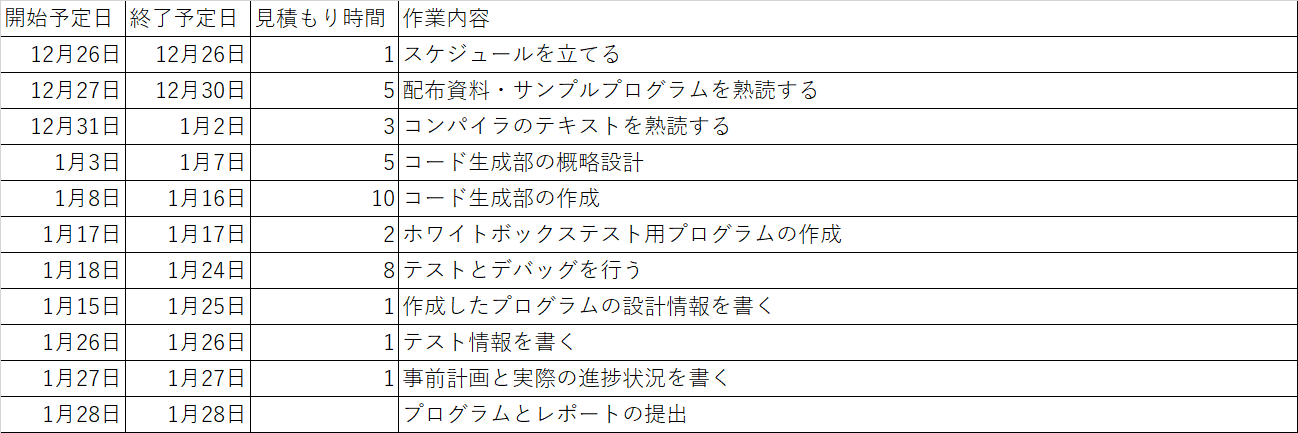
\includegraphics[scale=0.6]{kadai4_jizen.png}
\end{center}
\end{table}

しかし、演習中に計画を以下の表\ref{tb:shusei}のように修正した。
\begin{table}[H]
\begin{center}
\caption{課題4における修正後のスケジュール}
\label{tb:shusei}
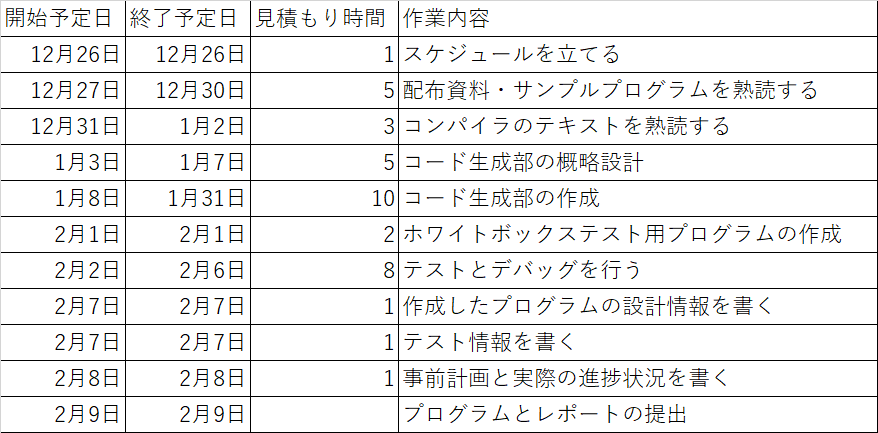
\includegraphics[scale=0.6]{kadai4_shusei.png}
\end{center}
\end{table}
\subsection{事前計画の立て方についての前課題からの改善点}
今回はアセンブリ言語の仕様など、理解すべき事項が多かったので、テキストの熟読の時間を長めに確保した。
\subsection{実際の進捗状況}
約3週間に及ぶ入院のため、大きく遅れを取ることになった。
\subsection{当初の事前計画と実際の進捗との差の原因}
上記の通り、約3週間怪我のため入院していたため、締め切りは伸ばしていただいたものの、コーディングが大幅に遅れを取ることとなった。
\end{document}
